\documentclass[12pt]{article}
\usepackage{titling}
\usepackage[shortlabels]{enumitem}
\usepackage[margin=0.8in]{geometry}
\usepackage{amsmath}
\usepackage{amssymb}
\usepackage{tabto}
\usepackage{setspace}
\usepackage{siunitx}
\usepackage{graphicx}
\usepackage{float}
\usepackage{tikz}
\usepackage{caption}

\title{CM20219 - CW 2 - 2020/21}
\preauthor{}
\author{}
\postauthor{}
\captionsetup[figure]{labelsep=space}
\begin{document}
\maketitle
\onehalfspacing
\section{Draw a simple cube}
The cube was drawn with side dimensions of 2. Since the default for $scene.add$ is to centre the cube
at the origin $(0,0,0)$, side lengths of 2 gives the corner coordinates $(-1,-1,-1)$ and $(1,1,1)$.
the $wireframe$ parameter simply makes the cube easier to see, and the $color$ is blue.
\begin{figure}[ht]  
    \centering
    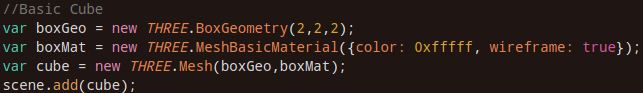
\includegraphics[width=10cm]{1.png}
    \label{fig:1}
    \caption{}
  \end{figure}
  \begin{figure}[ht]  
    \centering
    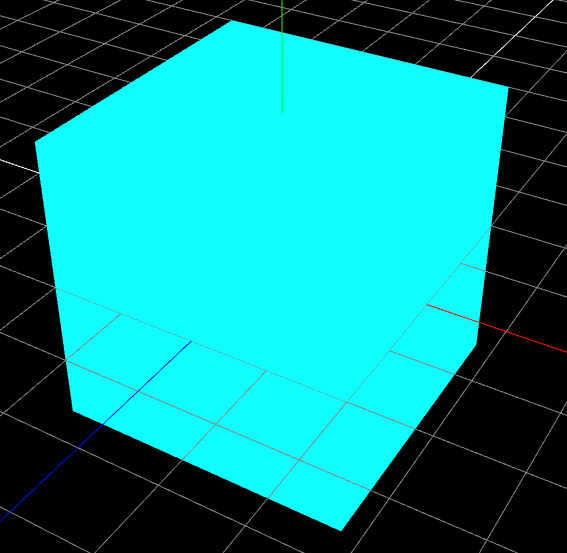
\includegraphics[width=5cm]{14.png}
    \label{fig:1}
    \caption{}
  \end{figure}
\section{Draw coordinate system axes}
The axes are simply drawn using the built-in $AxesHelper$ function.
\begin{figure}[ht]  
    \centering
    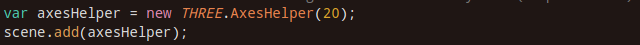
\includegraphics[width=10cm]{2.png}
    \label{fig:2}
    \caption{}
  \end{figure}
\section{Rotate the cube}
Rotation of the cube is performed by adjusting the object (cube) $rotation$ property. the $rotateCube()$ function is called in $animate()$ so that it is constantly updated.
\begin{figure}[H]  
    \centering
    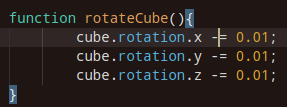
\includegraphics[width=5cm]{3.png}
    \caption{}
    \label{fig:3}
\end{figure}
\begin{figure}[H]  
    \centering
    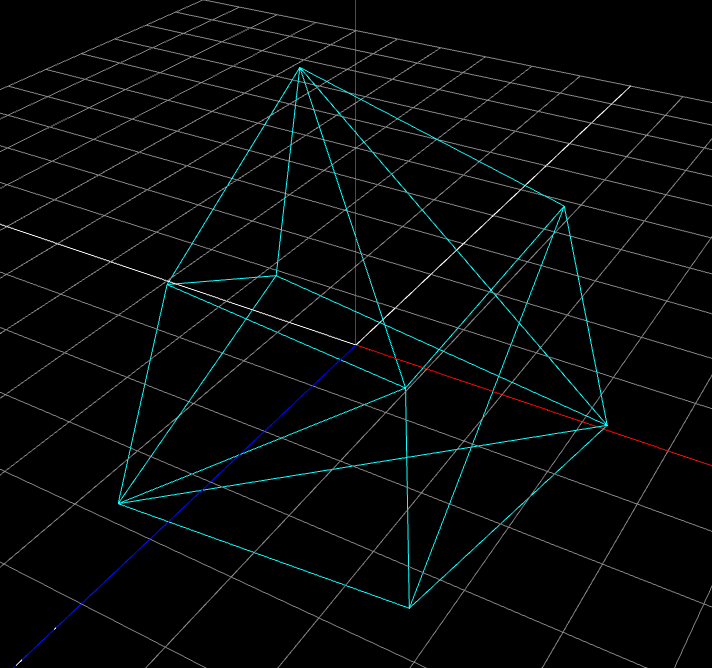
\includegraphics[width=10cm]{4.png}
    \caption{}
    \label{fig:4}
\end{figure}
As you can see in Figure \ref{fig:4}, the cube now rotates.
\section{Different Render Modes}
Switching render modes is done in the $handleKeyDown()$ function, as seen in Figure \ref{fig:5}. Each time either $v,e,f$ are pressed, a new $CubeGeometry$ is generated.
Faces are generated with the same code as requirement 1. The edges are drawn using $EdgeGeometry$ and vertices are drawn by using a $PointsMaterial$ along with $CubeGeometry$ in the mesh. Each
keypress starts with $scene.remove(cube)$, then the changes are made, then the cube is readded to the scene.
\begin{figure}[H]  
  \centering
  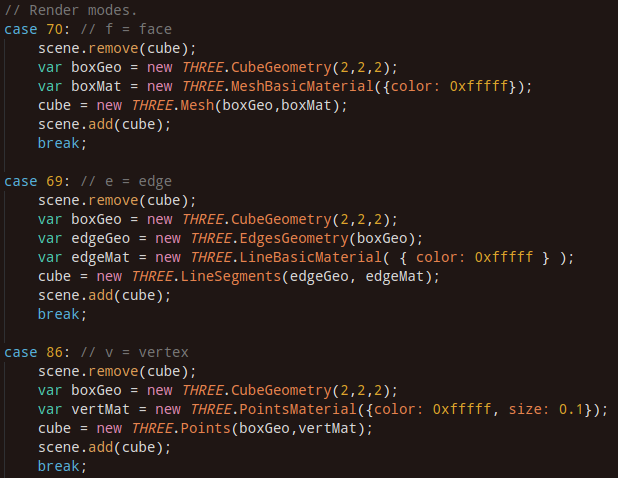
\includegraphics[width=10cm]{5.png}
  \caption{}
  \label{fig:5}
\end{figure}
\begin{figure}[H]  
  \centering
  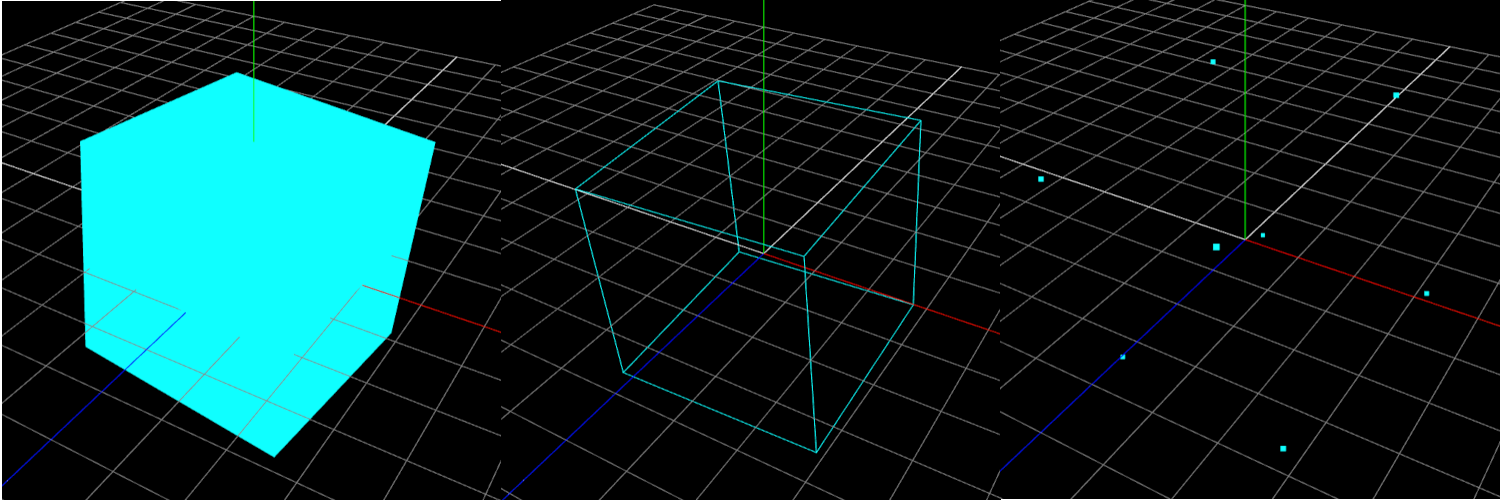
\includegraphics[width=\textwidth]{8910.png}
  \caption{}
  \label{fig:6}
\end{figure}
\section{Translate the Camera}
The camera is translated on its local axes using the arrow keys, as seen in Figure \ref{fig:7}. Backwards/forwards zooming is handled by
the scroll wheel, as seen in Figure \ref{fig:8}. In addition to the function shown in Figure \ref{fig:8}, A new $EventListener$ was added for the mouse wheel, just under the $EventListener$ for keypresses.
\begin{figure}[H]  
  \centering
  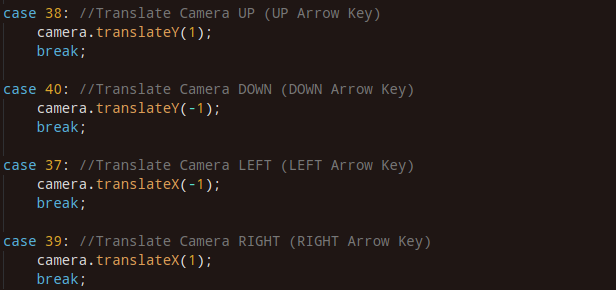
\includegraphics[width=10cm]{6.png}
  \caption{}
  \label{fig:7}
\end{figure}
\begin{figure}[H]  
  \centering
  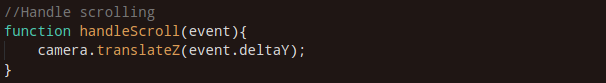
\includegraphics[width=10cm]{7.png}
  \caption{}
  \label{fig:8}
\end{figure}
\begin{figure}[H]  
  \centering
  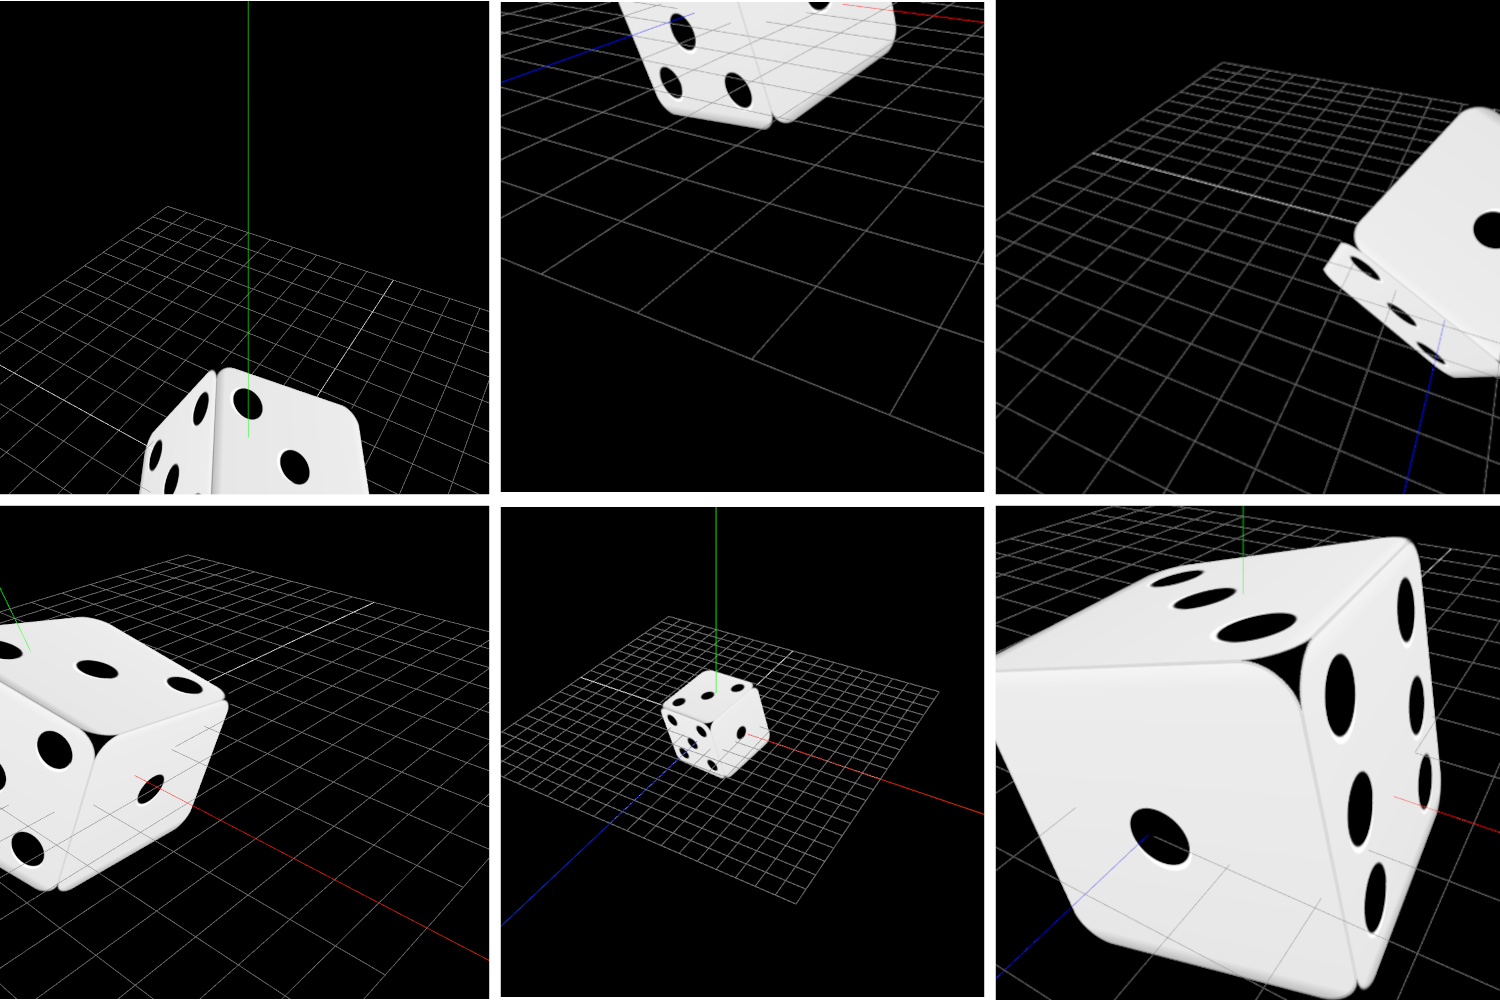
\includegraphics[width=10cm]{req5.png}
  \caption{}
  \label{fig:8}
\end{figure}
\section{Orbit the camera}
Camera orbiting is done using a click-and-drag motion. The button press is recorded when the mouse is pressed, and as the mouse moves, the spherical coordinates of the camera are recorded. The new position of the camera is then calculated using a triangle within the sphere; the hypothenuse being the radius of the circle. We have then have our two angles of rotation, theta and phi; theta is the angle between the plane $y=0$ and the radius, phi is the angle between the plane $x=0$ and the radius. 
\begin{figure}[H]  
  \centering
  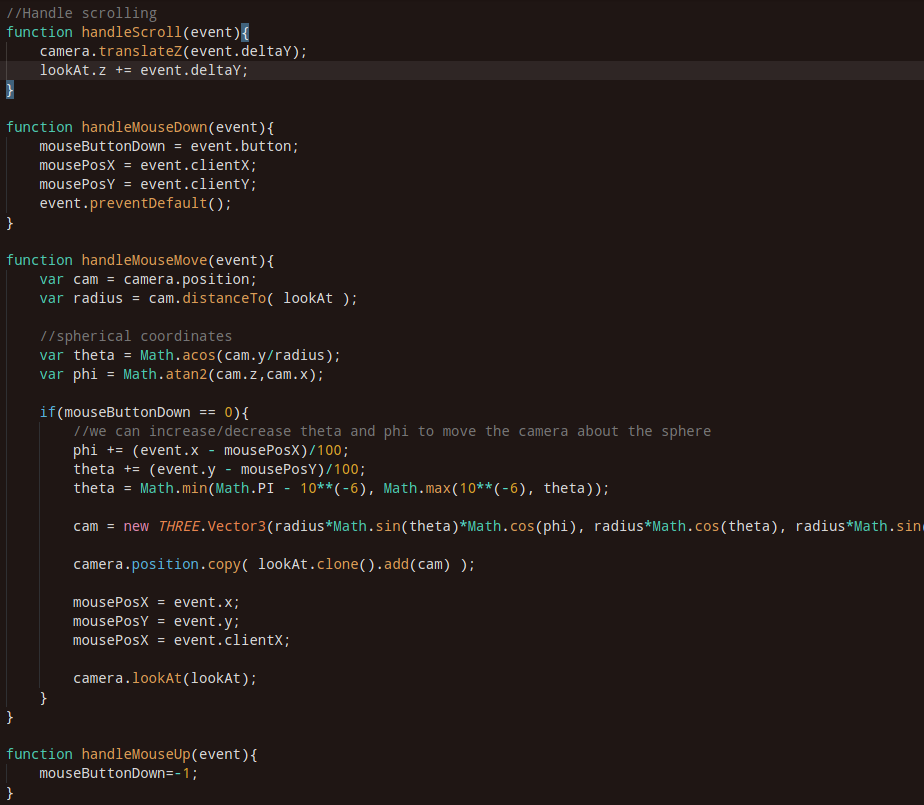
\includegraphics[width=10cm]{22.png}
  \caption{}
  \label{fig:15}
\end{figure}
As you can see in Figures \ref{fig:test5},\ref{fig:test4} and \ref{fig:tes0t4}, the camera is able to move freely.
\begin{figure}[H]
  \centering
  \begin{minipage}{.33\textwidth}
    \centering
    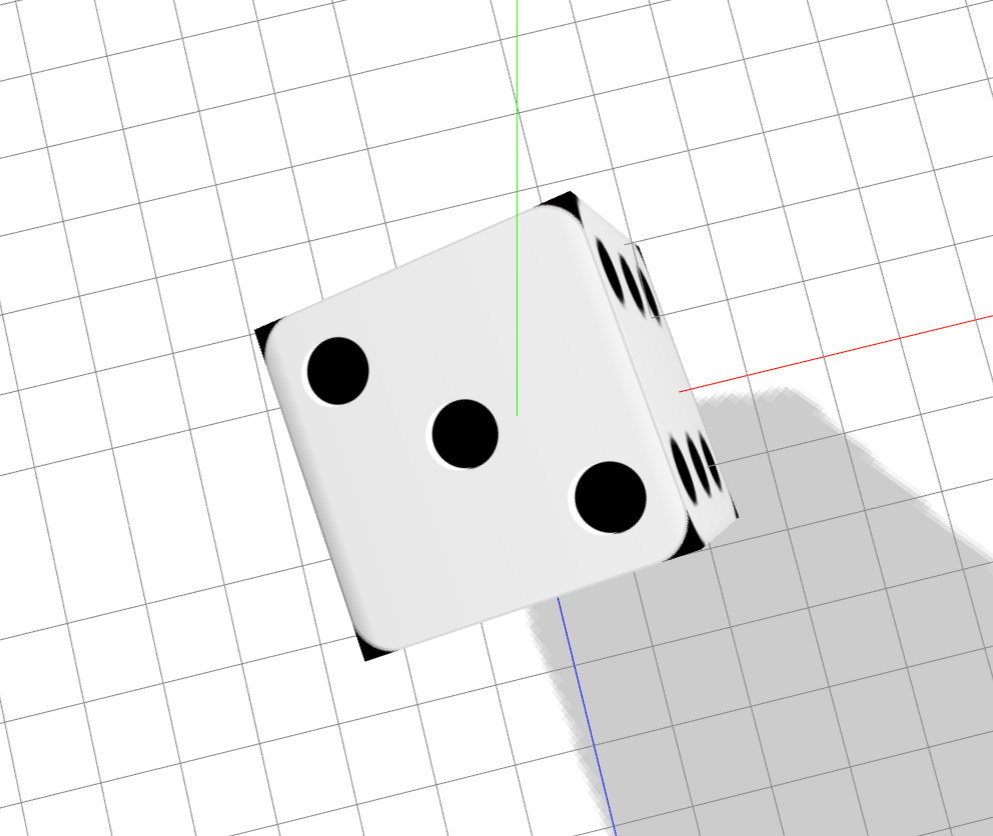
\includegraphics[width=.9\linewidth]{23.png}
    \captionof{figure}{}
    \label{fig:test5}
  \end{minipage}%
  \begin{minipage}{.33\textwidth}
    \centering
    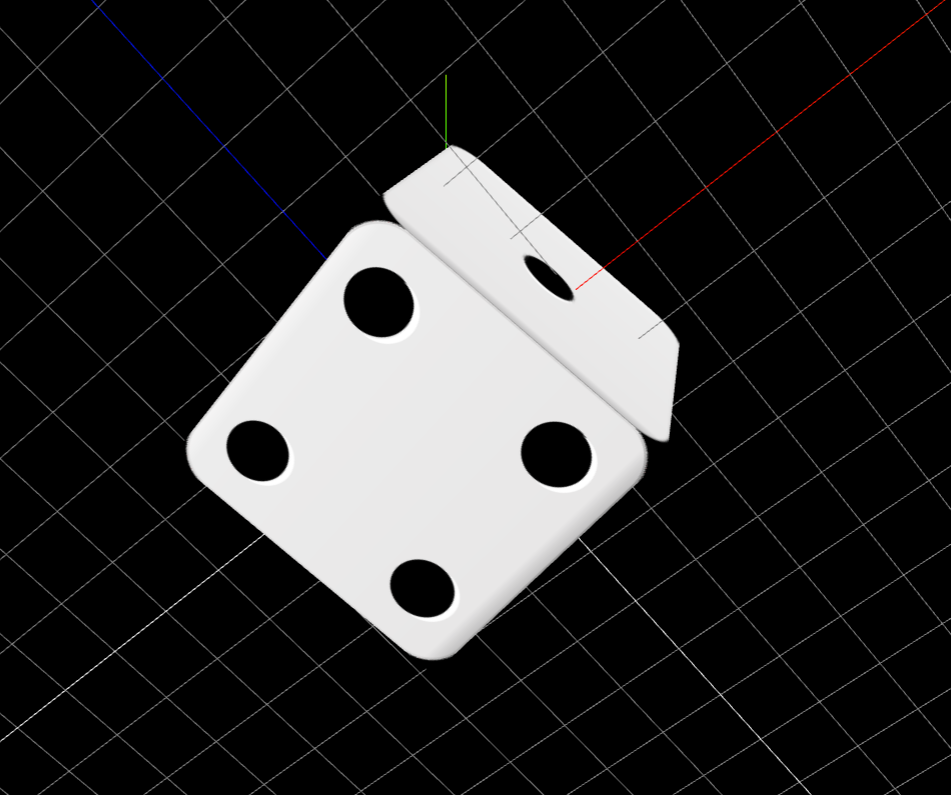
\includegraphics[width=.9\linewidth]{24.png}
    \captionof{figure}{}
    \label{fig:test4}
  \end{minipage}
  \begin{minipage}{.33\textwidth}
    \centering
    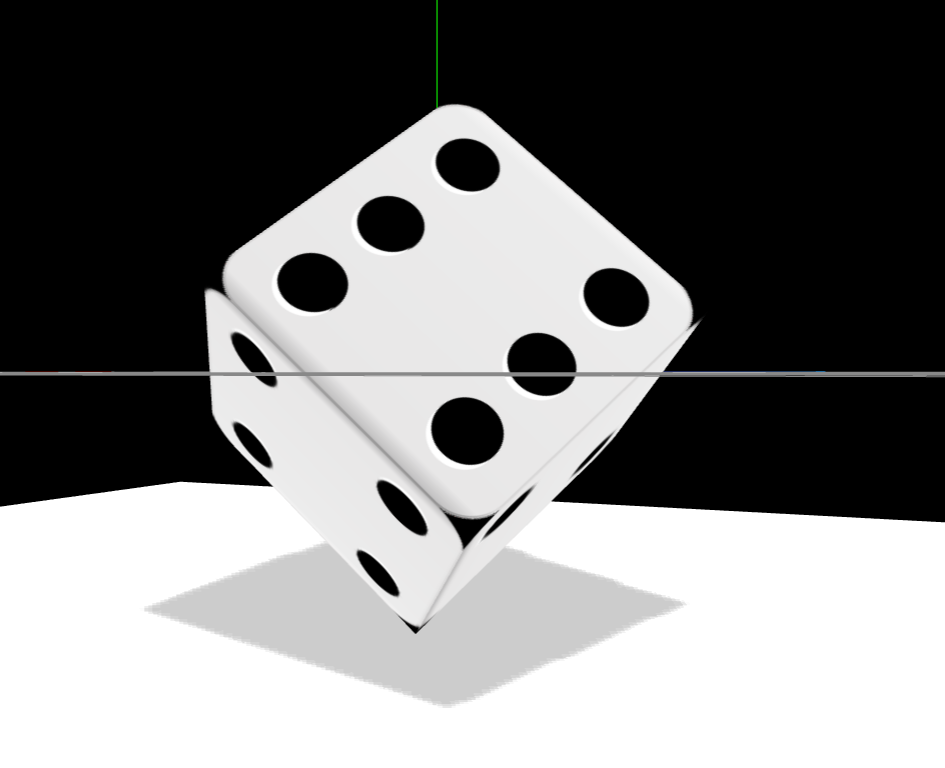
\includegraphics[width=.9\linewidth]{25.png}
    \captionof{figure}{}
    \label{fig:tes0t4}
  \end{minipage}
\end{figure}
Unfortunately, I was not able to fully figure out how to adjust the lookAt position based on the translation of the camera, and the functionality is a little bit patchy and it tends to get into some form of gimbal lock. I suspect this is because when I translate the camera, I simply change the respective lookAt axis coordinate by the same amount, however the camera is moving on its local axes, whereas lookAt is on the global axes.
If I had time I would be able to properly implement this.
\section{Texture mapping}
Textures are loaded using the built-in $TextureLoader$, then mapped onto each face of the cube. The function $createDiceTexture()$ is then called from $init()$, as well as every time the user switches to face rendering mode. The dice texture is seen in Figure \ref{fig:14}.
\begin{figure}[H]
  \centering
  \begin{minipage}{.5\textwidth}
    \centering
    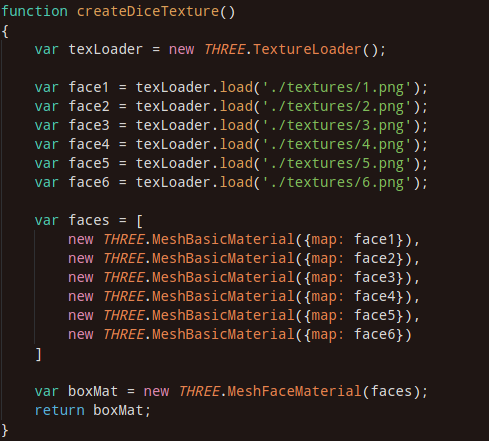
\includegraphics[width=.9\linewidth]{11.png}
    \captionof{figure}{}
    \label{fig:9}
  \end{minipage}%
  \begin{minipage}{.5\textwidth}
    \centering
    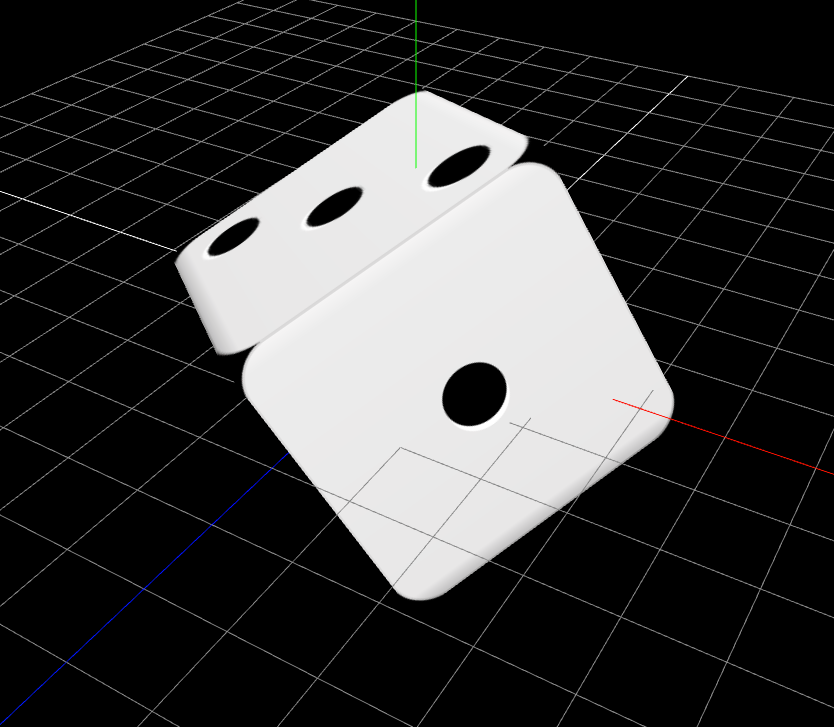
\includegraphics[width=.9\linewidth]{15.png}
    \captionof{figure}{}
    \label{fig:14}
  \end{minipage}
\end{figure}
\section{Load a mesh model from .obj}
To load the Object from the .obj file, I chose to switch to a 'module' type script, as this was the easiest way to include $OBJLoader$. As a result, I had to download and include $three.module.js$ instead of the original $three.js$ file provided. Additionally, I took the most recent $OBJLoader.js$ version from the project's GitHub.
2 import statements had to be included at the start of the script, as can be seen in Figure \ref{fig:10}.
\begin{figure}[H]  
  \centering
  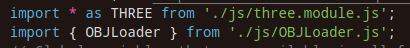
\includegraphics[width=10cm]{13.png}
  \caption{}
  \label{fig:10}
\end{figure}
I then created the function $loadBunny()$, seen in Figure \ref{fig:11}. It uses $OBJLoader$'s $load()$ function, which takes the name of the .obj file as an argument, as well as function to be run upon loading. There are optional parameters to include functions for errors and such, but I chose not to include these.
The object was then scaled to fit inside the cube by setting the $scale$ property for all dimensions. I chose 0.3 as the scale factor as this seemed to work. The new object is then loaded into the scene as usual with $scene.add()$. I set $bunny = object$ as $bunny$ is a global variable, which comes in handy later when performing operations on the object for the different rendering modes stated in Requirement 9.
\begin{figure}[H]  
  \centering
  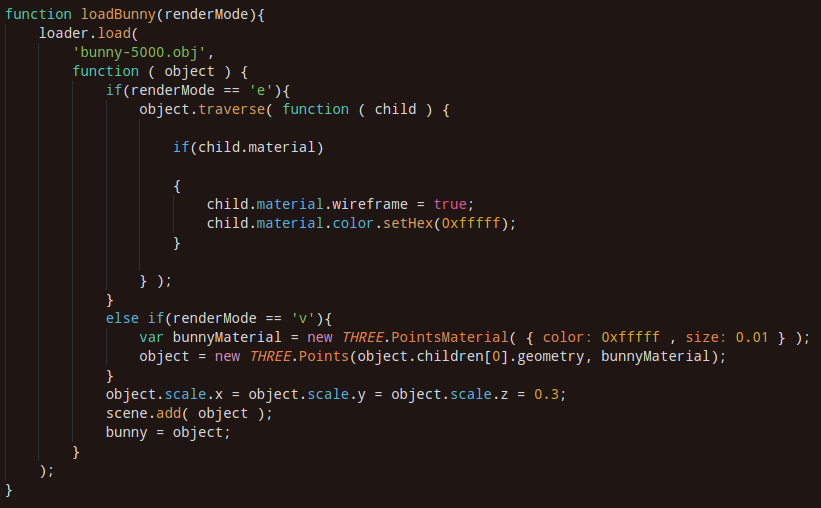
\includegraphics[width=15cm]{12.png}
  \caption{}
  \label{fig:11}
\end{figure}
\section{Rotate the mesh, render it in different modes}
The bunny is rotated in exactly the same way as the cube; a function $rotateBunny()$ is created, the same as Figure \ref{fig:3}, but with $bunny$ instead of $cube$. This new function is then included in $animate()$.
Rendering is done by the $loadBunny()$ function, which is called with an optional parameter in the same location the rendering modes for the cube are done. For face mode, no parameter is included so the bunny is just loaded in. For edges, 'e' is passed, in which case after loading, the object is traversed and the materials of the children are set to wireframe (and colour set to blue too). For vertices mode, a $PointsMaterial$ is created the same as for cube, and the object is set to a $Points$ object, with the objects mesh geometry used.
\begin{figure}[H]  
  \centering
  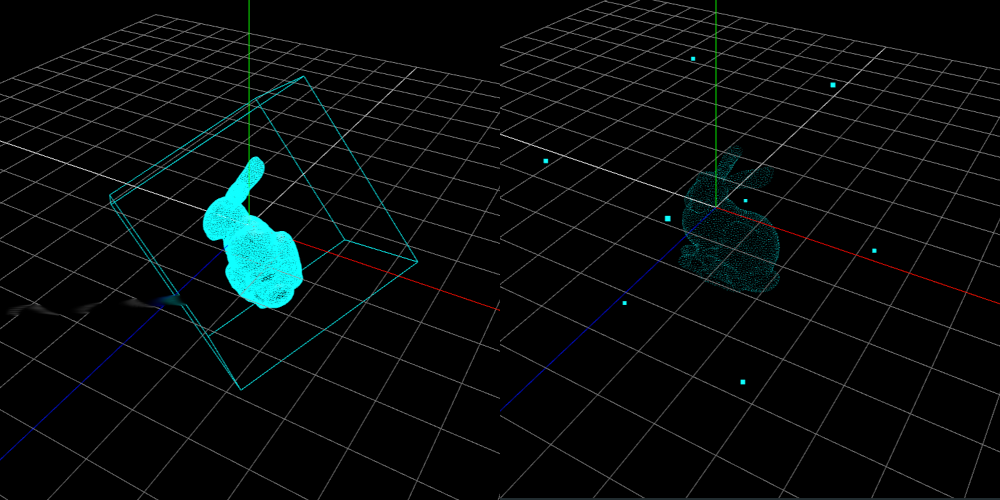
\includegraphics[width=10cm]{18.png}
  \caption{}
  \label{fig:12}
\end{figure}
\section{Be creative - Shadows}
For Requirement 10 I decided to create a plane and cast shadows from the cube onto it. The plane was created,
and then placed horizontally at $y=-2$, so that it wouldn't overlap the cube. A light source was then created, and a few settings were changed 
such as on the renderer and the cube so that they would render or cast/receive shadows. The result is Figure \ref{fig:13}.
\begin{figure}[H]
  \centering
  \begin{minipage}{.5\textwidth}
    \centering
    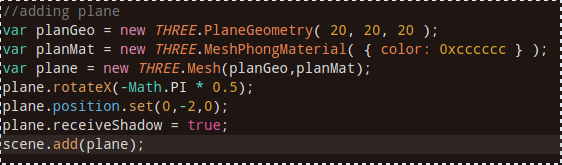
\includegraphics[width=.9\linewidth]{19.png}
    \captionof{figure}{}
    \label{fig:test1}
  \end{minipage}%
  \begin{minipage}{.5\textwidth}
    \centering
    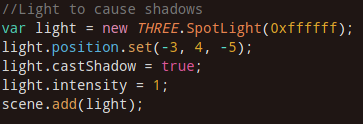
\includegraphics[width=.9\linewidth]{20.png}
    \captionof{figure}{}
    \label{fig:test2}
  \end{minipage}
  \end{figure}
  \begin{figure}[H]  
    \centering
    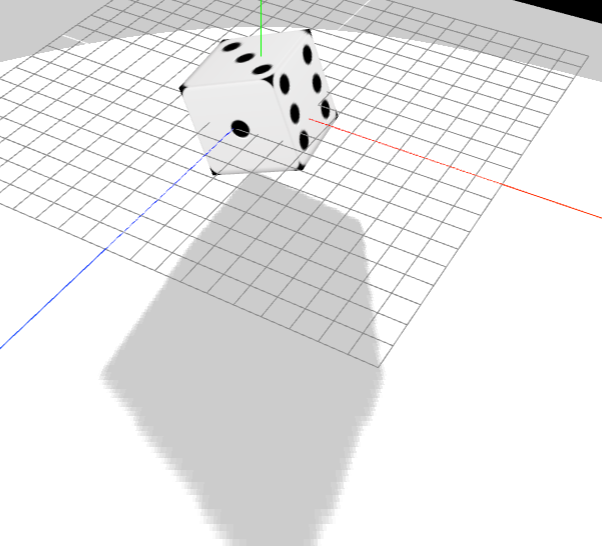
\includegraphics[width=6cm]{21.png}
    \caption{}
    \label{fig:13}
  \end{figure}
\section{Evaluation}
Given more time, I would be able to improve the general code quality as there is little code reuse currently, and implement more solid test coverage. I would also be able to fix the issues mentioned under Requirement 6.

\end{document}